В секции будут рассмотрена формальная вычислительная теория языка.
Подход был предложен Ноамом Хомски разработанной для разработки
в его работе "Синтаксические структуры" \cite{chomsky2002syntactic}. Направление изучает алгоритмические 
методы по изменению морфемного состава слова, формированию представления о связи слов в тексте.

Введем ключевые предметные определения, позволяющие формализовать анализ и 
синтез предложений в естественном языке, что важно для многих приложений 
в области обработки естественного языка и вычислительной лингвистики.
 
\textit{Определение} Формального языка является совокупностью:
\begin{itemize}
    \item \textit{алфавита} $\Sigma$ - конечного множества символов, из которых строятся строки языка.
    \item \textit{строки} - последовательности символов из алфавита, которые принадлежат языку.
    \item \textit{грамматики} - набора правил, которые определяют, какие строки являются допустимыми в языке.
\end{itemize}
\begin{figure}[h]
    \centering
    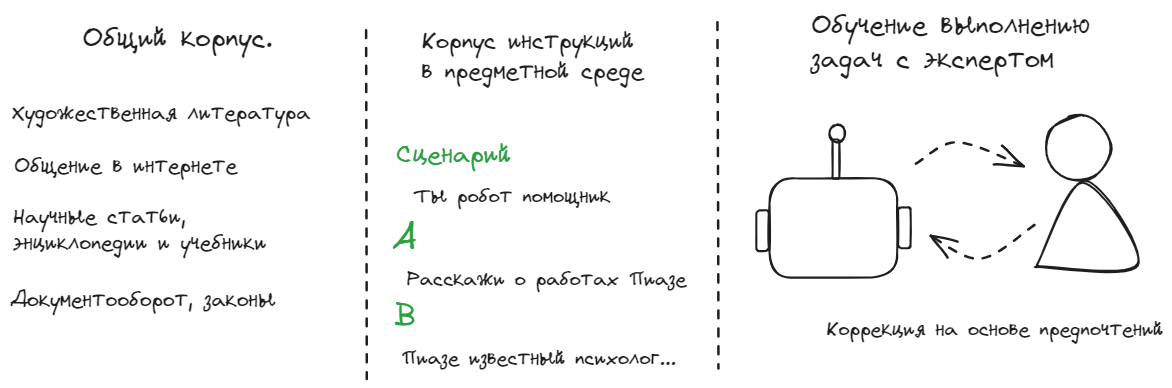
\includegraphics[width=0.5\textwidth]{assets/work/arch/learning.excalidraw.png}
    \caption{Обучение разбито на три ключевых этапа: подготовка, адаптация на корпусе}
    \label{train}
\end{figure}

\textit{Определение} Автоматом называется:
\begin{itemize}
    \item \textit{алфавита} $\Sigma$ - конечного множества символов, из которых строятся строки языка.
    \item \textit{строки} - последовательности символов из алфавита, которые принадлежат языку.
    \item \textit{грамматики} - набора правил, которые определяют, какие строки являются допустимыми в языке.
\end{itemize}


\textit{Определение} \textbf{Формальный язык} — строго определённое множество строк $S$, составленных из конечного алфавита символов $\Omega$,
 которые подчиняются определённым правилам или грамматике.
Эти правила определяют синтаксис языка, то есть допустимые последовательности символов,
 и часто могут быть представлены с помощью формальных грамматик, таких как контекстно-свободные или регулярные грамматики.

Для определения синтаксических связей как правило используют графовые методы.

\textit{Определение} \textbf{Синтаксическое дерево}(parse tree) описывается как взаимодействие между \begin{itemize}
    \item упорядоченным деревом $T$, которое представляет синтаксическую структуру предложения.
    \item синтаксической категории (например, S, NP, VP), либо терминальному символу, присеваемому множеству вершин дерева $T$ $N$ . 
    \item корню дерева $T$  $r$, обозначающем всю структуру предложения. 
    \item Листья представляют собой слова в предложении. Листья** $L \subseteq N$ — это узлы, которые не имеют дочерних узлов. 
    \item Cинтаксические категории или промежуточные составляющие, соответствующие $I = N \setminus L$ — это узлам, у которых имеется хотя бы одного потомка. 
\end{itemize}

Тогда дерево разбора $T$ для строки $w = w_1 w_2 \ldots w_n$ запишется как четверка $T = (N, E, r, L)$, где \begin{itemize}
    \item $N$ — конечное множество узлов,
    \item $E \subseteq N \times N$ — множество ребер, каждое из которых соединяет пару узлов (родитель — потомок),
    \item  $r \in N$ — корень дерева,
    \item $L = \{ w_1, w_2, \ldots, w_n \} \subseteq N$ — множество листьев, соответствующих словам в предложении.
\end{itemize}


\textit{Определение} \textbf{Морфологическим анализом} называют процесс разложения 
слова $w$ на его морфемы, например, префикс $P$, корень $R$ и суффикс $S$, из словаря $S$

\textit{Определение} \textbf{Морфологическим синтезом} называется функция $f$,
формирующая слова $w$ из леммы $l$ и морфологических характеристик $m$. 
Примерами морфологических характеристик являются число, род, падеж.
 
\textit{Определение} \textbf{Правилами словообразования} называют ограничения,
 определяющие трансформации между леммами и словоформами. 
 Пусть \( T \) — множество таких правил. Каждое правило \( t \in T \) можно представить в виде
 $t: (l, m) \rightarrow w$

\textit{Определение} \textbf{Лексикон} называется декартово произведение лемм 
из словаря $\Sigma$ и возможных атрибутов $A$. $L = \Sigma \times A$
 

\textit{Определение} \textbf{Формальная грамматика} задается четверкой
$ G  = \left(N, \Sigma, R, S\right)$, где $N$ — множество нетерминальных символов, 
$\Sigma$ — множество терминальных символов, 
$R$ — множество правил, 
$S$ — стартовый символ.
 
 
 Эти формальные выражения и определения дают основу для создания и анализа алгоритмов в вычислительной морфологии, обеспечивая строгую и систематическую обработку естественного языка.




 
 


